\documentclass{article}
\usepackage{aaai17}
\usepackage{amsmath}
\usepackage{graphicx}
\usepackage{verbatim}
\graphicspath{ {images/} }
\frenchspacing
\setlength{\pdfpagewidth}{8.5in}
\setlength{\pdfpageheight}{11in}

\title{
	CS4246 Project 1\\ Depression Prediction
}
\author{
	{\bf Team 01} \\
	Antoine Charles Vincent Garcia - A0159072A\\
	Chan Jun Wei - A0112084\\
	Chen Tze Cheng - A0112092\\
	Eric Ewe Yow Choong - A0112204\\
	Han Liang Wee, Eric - A0065517\\
	Ho Wei Li - A0094679\\
}

\begin{document}
 	\maketitle

	\begin{abstract}
	\begin{quote}
	In this report, we illustrate the use of Gaussian Processes to calculate and model stress levels in society and with the data obtained, is used to estimate depression severity.
	\end{quote}
	\end{abstract}
	
	\section{Introduction}

	\section{Gaussian Process Regression Model}

	\section{Technical Approach}

	\section{Evaluation}
	In order to test our Gaussian Process model, we conducted tests on data obtained from Audio/Visual Emotion Challenge and Workshop(AVEC 2016). The goal of AEVC is to weigh-in on the various approaches(visual, audio) used to recognize emotions under unambiguous conditions. AVEC 2016 provided 2 pieces of data as input: visual and auditory data. However, we would be reducing the scope of the experiment, limiting the experiment to only the auditory data. Two Sub-Challenges are lised in AVEC 2016. We are only interested in the Depression Classification Sub-Challenge, which requires participants to classify inputs by the PHQ-8 score.

	\subsection{Data}
	The depression data used in AVEC 2016 was obtained from the benchmarking database, the Distress Analysis Interview Corpus - Wizard of Oz(DAIC-WOZ). Data collected from DAIC-WOZ include audio and video recordings and the corresponsing PHQ-8 score[CITE:27](0-24), which is a frequently used self-report scheme to access severity of depression[CITE]. Henceforth, we would need to pre-process the auditory data before we use it in our Gaussian Process Model. The data is pre-processed as described in the Section [REF]. The distribution of the depression severity scores in both training and development set is given in Figure \ref{histogram_phq8}. The data provided are split into 2 sets: training and development. A summary of the data is given in Table \ref{summary_table}.
	\begin{figure}
  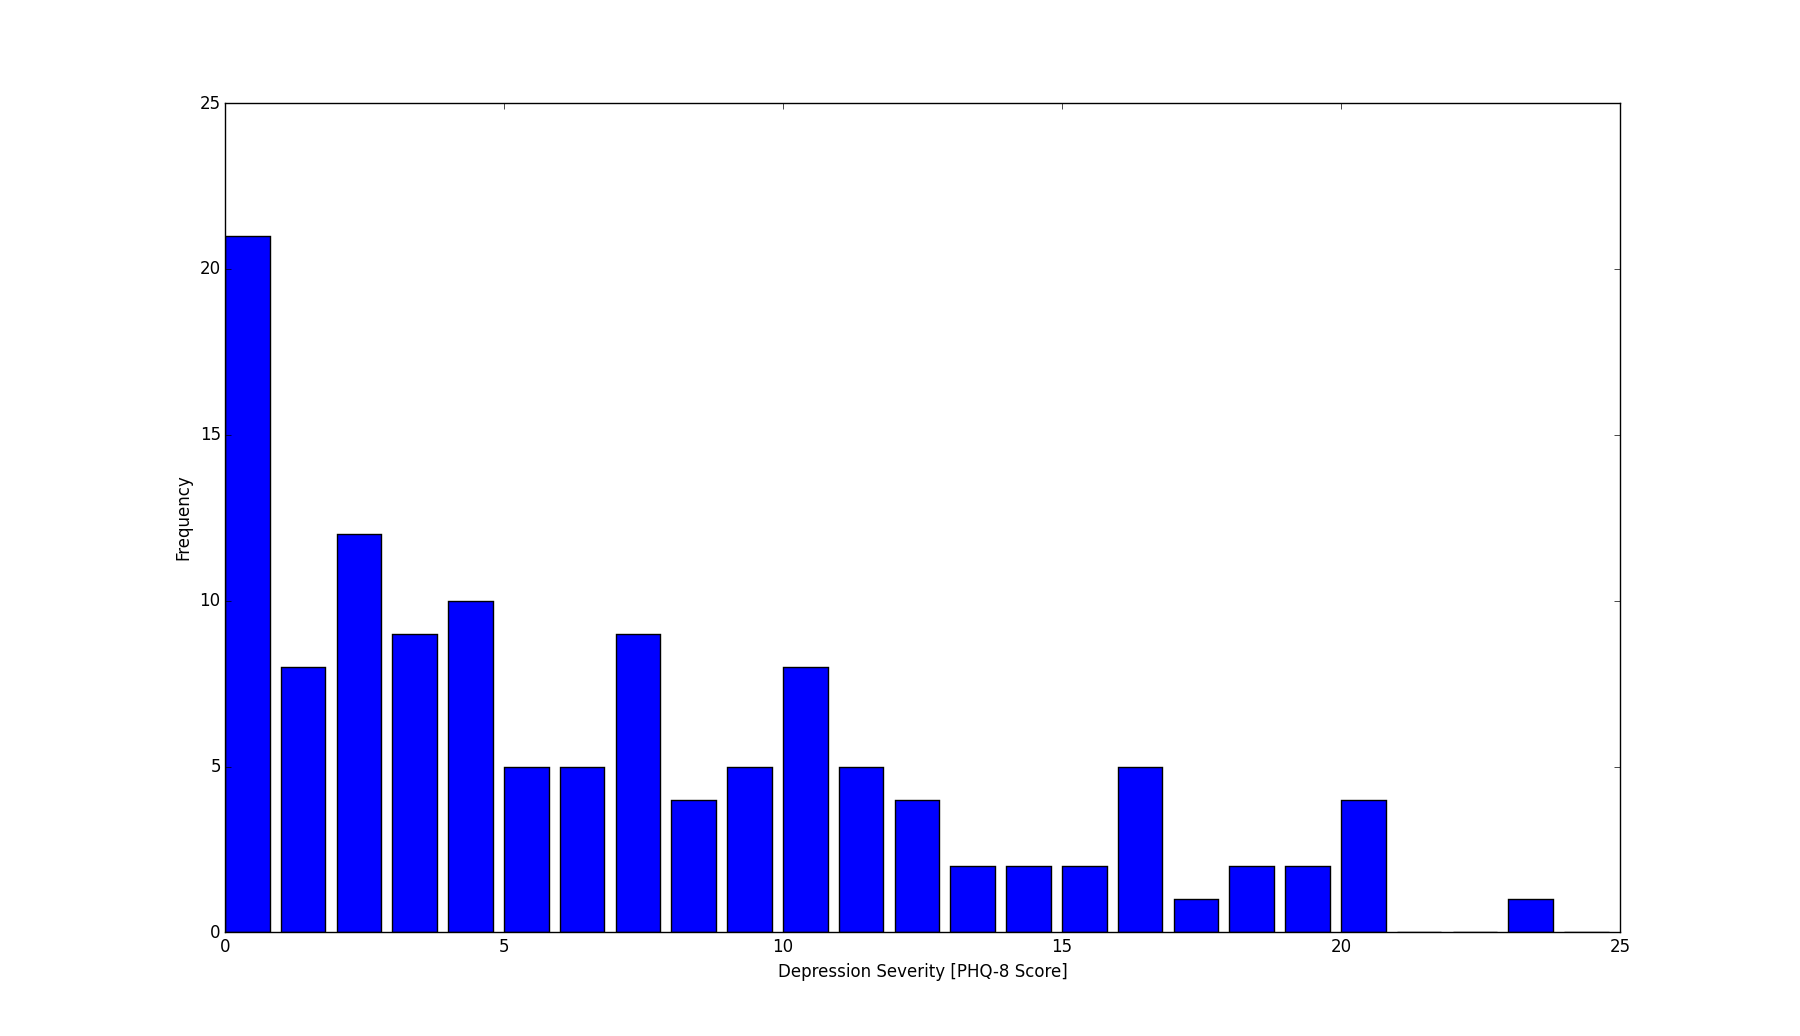
\includegraphics[width=0.45\textwidth]{histogram_phq8}
  \caption{PHQ-8 scores' histogram of both training and development set}
  \label{histogram_phq8}
 \end{figure}
 \subsection{Measure of Accuracy}
 AVEC 2016 provided a baseline classifier that consistently predicts the PHQ-8 score with $\text{RMSE}=6.7418$[CITE]. In order to provide a meaningful and consistent comparison to the baseline provided, we would be only using Root Mean Square Deviation Error(RMSE) to measure the error rate on both Training and Development datasets. RMSE(Equation \ref{eq:rmse}) is a commonly used in machine learning communities to measure the differences between the values predicted by a model and the values actually observed. 

 \begin{equation}\label{eq:rmse}
  \text{RMSE} = \sqrt{\frac{\sum_{t=1}^n (\hat y_t - y_t)^2}{n}}
 \end{equation}
 \begin{table}
  \begin{center}
   \begin{tabular}{ | r | c | c || c | }
    \hline
    & Training & Development & All \\ \hline
    n               & 95 & 31 & 126 \\ \hline
    $\mu$           & 6.326 & 7.548 & 6.626 \\ \hline
    $\sigma$        & 5.597 & 6.690 & 5.909 \\ \hline
   \end{tabular}
  \end{center}
  \caption{Summary of Datasets provided}
  \label{summary_table}
 \end{table}
 [CITEDBLP:journals/corr/ValstarGSRLTSSC16]
 
 \subsection{Experimental Setup}
 We compared our Gaussian Model against commonly used machine learning algorithms. The list of algorithms and their hyperparameters are given in Table \ref{list_mls}. The hyper-parameters are either determined by the defaults used in the popular machine learning library, Scikit Learn[CITE] or some reasonable values were used. Each machine learning algorithm is trained against the training set and thereafter tested against the development set using RMSE as the error metric. The process used is shown in Figure \ref{process}.
	\begin{figure}
 	\begin{center}
   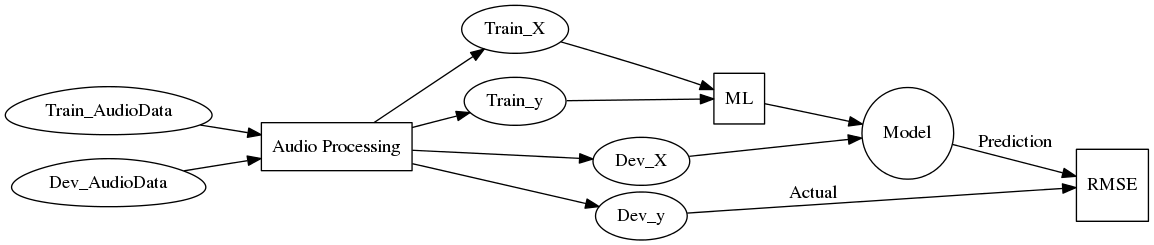
\includegraphics[width=0.25\textwidth]{process}
  \end{center}
  \caption{Experimental process}
  \label{process}
 \end{figure}
 \begin{comment}
 DO NOT REMOVE
 @startuml
 digraph g {
     ML,RMSE[shape=square];
     Model[shape=circle];
	 Train_X -> ML;
	 Train_y -> ML;
	 ML -> Model
	 Dev_X -> Model
	 Model -> RMSE[label=Prediction]
	 Dev_y -> RMSE[label=Actual]
	 RMSE -> Score
 }
 @enduml
 \end{comment}

 \begin{table}
  \begin{center}
   \begin{tabular}{ | r | c |}
    \hline
     Algorithm & Hyper-parameters \\ \hline\hline
    K-Nearest Neighbors        & x \\ \hline
    Linear SVM                 & x \\ \hline
    RBF SVM                    & x \\ \hline
    Decision Tree              & x \\ \hline
    Random Forest              & x \\ \hline
    AdaBoost                   & x \\ \hline
    Naive Bayes                & x \\ \hline
    Decision Tree              & x \\ \hline
   \end{tabular}
  \end{center}
  \caption{List of Machine Learning Algorithms with their corresponding hyper-parameters}
  \label{list_mls}
 \end{table}
 \subsection{Results}
 The results of the experiment is shown in t
 
 \begin{table}
  \begin{center}
   \begin{tabular}{ | r | c | c |}
    \hline
    & \multicolumn{2}{c|}{RMSE} \\ \hline
     Algorithm & Training & Development \\ \hline\hline
    K-Nearest Neighbors        & x & x \\ \hline
    Linear SVM                 & x & x \\ \hline
    RBF SVM                    & x & x \\ \hline
    Decision Tree              & x & x \\ \hline
    Random Forest              & x & x \\ \hline
    AdaBoost                   & x & x \\ \hline
    Naive Bayes                & x & x \\ \hline
    Decision Tree              & x & x \\ \hline
    Gaussian Process           & x & x \\ \hline
   \end{tabular}
  \end{center}
  \caption{RMSE results of the different machine learning algorithms}
  \label{rmse_results}
 \end{table}
 
 \begin{figure*}
  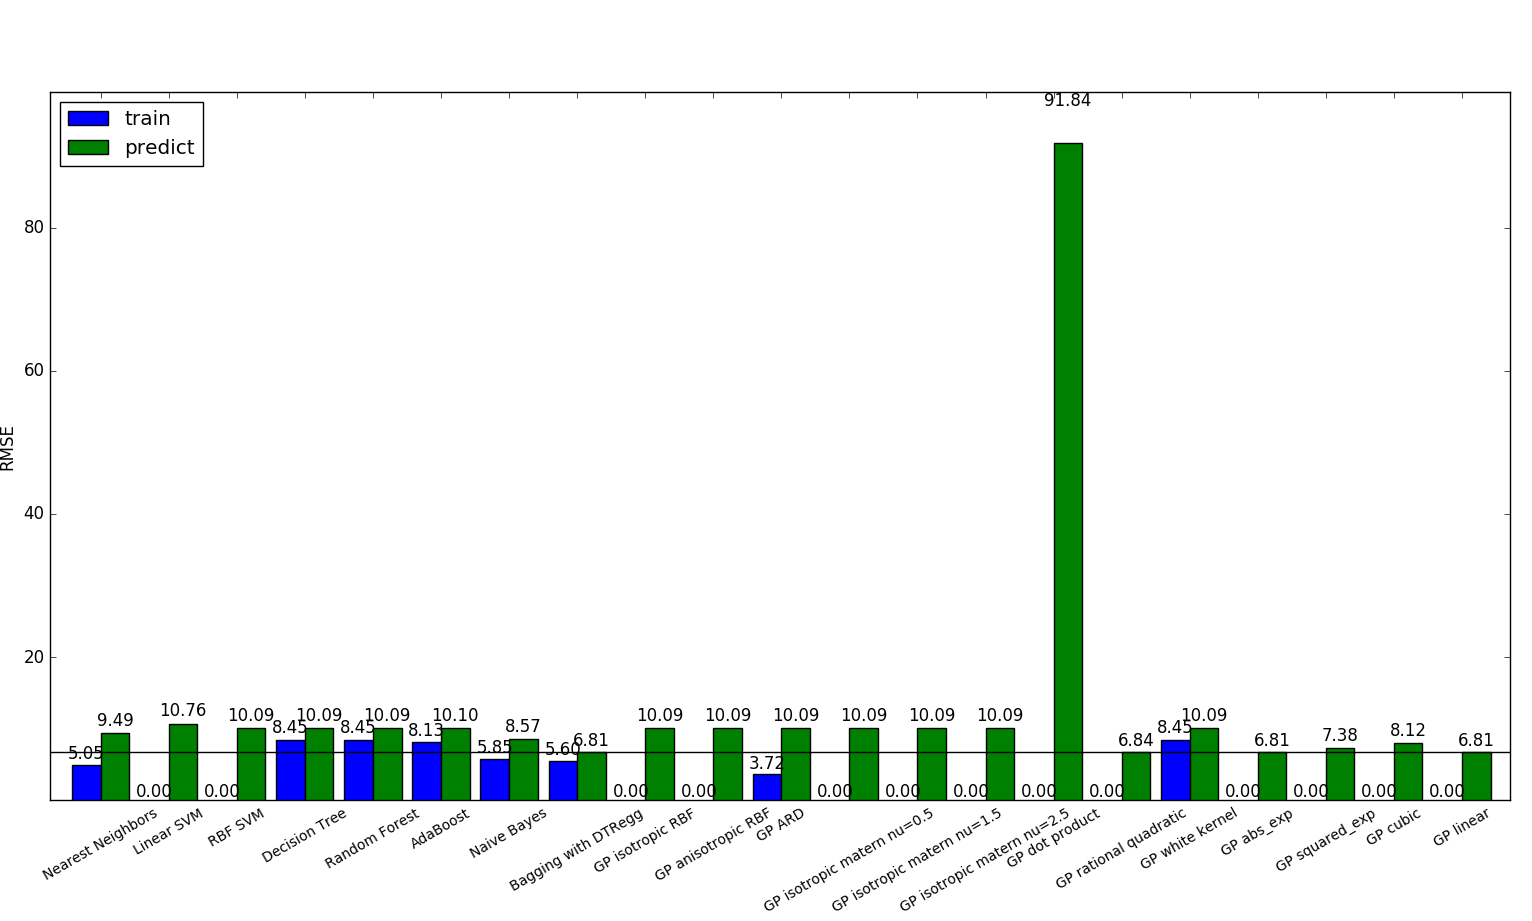
\includegraphics[width=\textwidth]{results}
  \caption{Chart showing RMSE(Training and Development) for the different classifiers}
  \label{rmse_results_chart}
 \end{figure*}
	\section{Conclusion}	


	\section{Main Roles of Each Member}
	\begin{itemize}
		\item \textbf{Antoine Charles Vincent Garcia}: 
		Scripting the program, setting up machine learning libraries and running tests.
		\item \textbf{Chan Jun Wei}: 
		Project technicalities such as problem formulation and modelling, mathematics and experiment planning.
		\item \textbf{Chen Tze Cheng}: 
		Project technicalities such as problem formulation and modelling, mathematics and experiment planning.
		\item \textbf{Eric Ewe Yow Choong}: 
		Documentation especially writing of the motivation, recording research findings and keeping track of requirements.
		\item \textbf{Han Liang Wee, Eric}: 
		Scripting the program, setting up machine learning libraries and running tests.
		\item \textbf{Ho Wei Li}: 
		Documentation especially writing up the motivation, recording research findings and keeping track of requirements.
	\end{itemize}
	
	\section{References}

\end{document}
